\documentclass[aspectratio=169,10pt]{beamer}
\usetheme{default}
\usecolortheme{seahorse}
\setbeamertemplate{navigation symbols}{}
\setbeamertemplate{footline}[frame number]
\usepackage{graphicx, booktabs}
\graphicspath{{../figures/}}
\title{Y-88 Energy Calibration, Gain Curves, and Trigger Thresholds}
\subtitle{n\_TOF EAR2 X17 --- Y-88 source scan (224476--79) + long run 224503}
\author{Dylan Neff \\[0.5ex] {\small analysis and slides prepared with Claude (Anthropic AI assistant)}}
\date{July 19, 2026}

\begin{document}

\begin{frame}\titlepage\end{frame}

\begin{frame}{What we did}
\begin{itemize}
\item \textbf{Y-88 source scan} (224476--79, one source per arm): an absolute
      energy calibration from the \textbf{699 \& 1612 keVee Compton edges},
      on plastics, liquids, and SiPM walls.
\item Reprocessed with the LIQ PSA UserInput (the official files have no LIQ).
\item Anchored the two \textbf{plastic HV scans} (224466 BNC-T, 224489 FIFO) to
      the Y-88 scale $\to$ absolute gain curves for setting HV.
\item \textbf{Long run 224503}: SiPM MIP (per arm) and plastic triple MIP recheck.
\item \textbf{Two significant discrepancies found} (flagged, need follow-up).
\item Deliverable: \textbf{trigger threshold estimates} for SiPM sums and plastics.
\end{itemize}
\vfill
{\small Scripts \texttt{21--23f}; docs \texttt{HV\_GAIN\_Y88\_ANALYSIS.md},
\texttt{report/y88\_report.pdf}.}
\end{frame}

\begin{frame}{Y-88 absolute scale: both Compton edges, all three detectors}
\begin{columns}
\column{.5\textwidth}
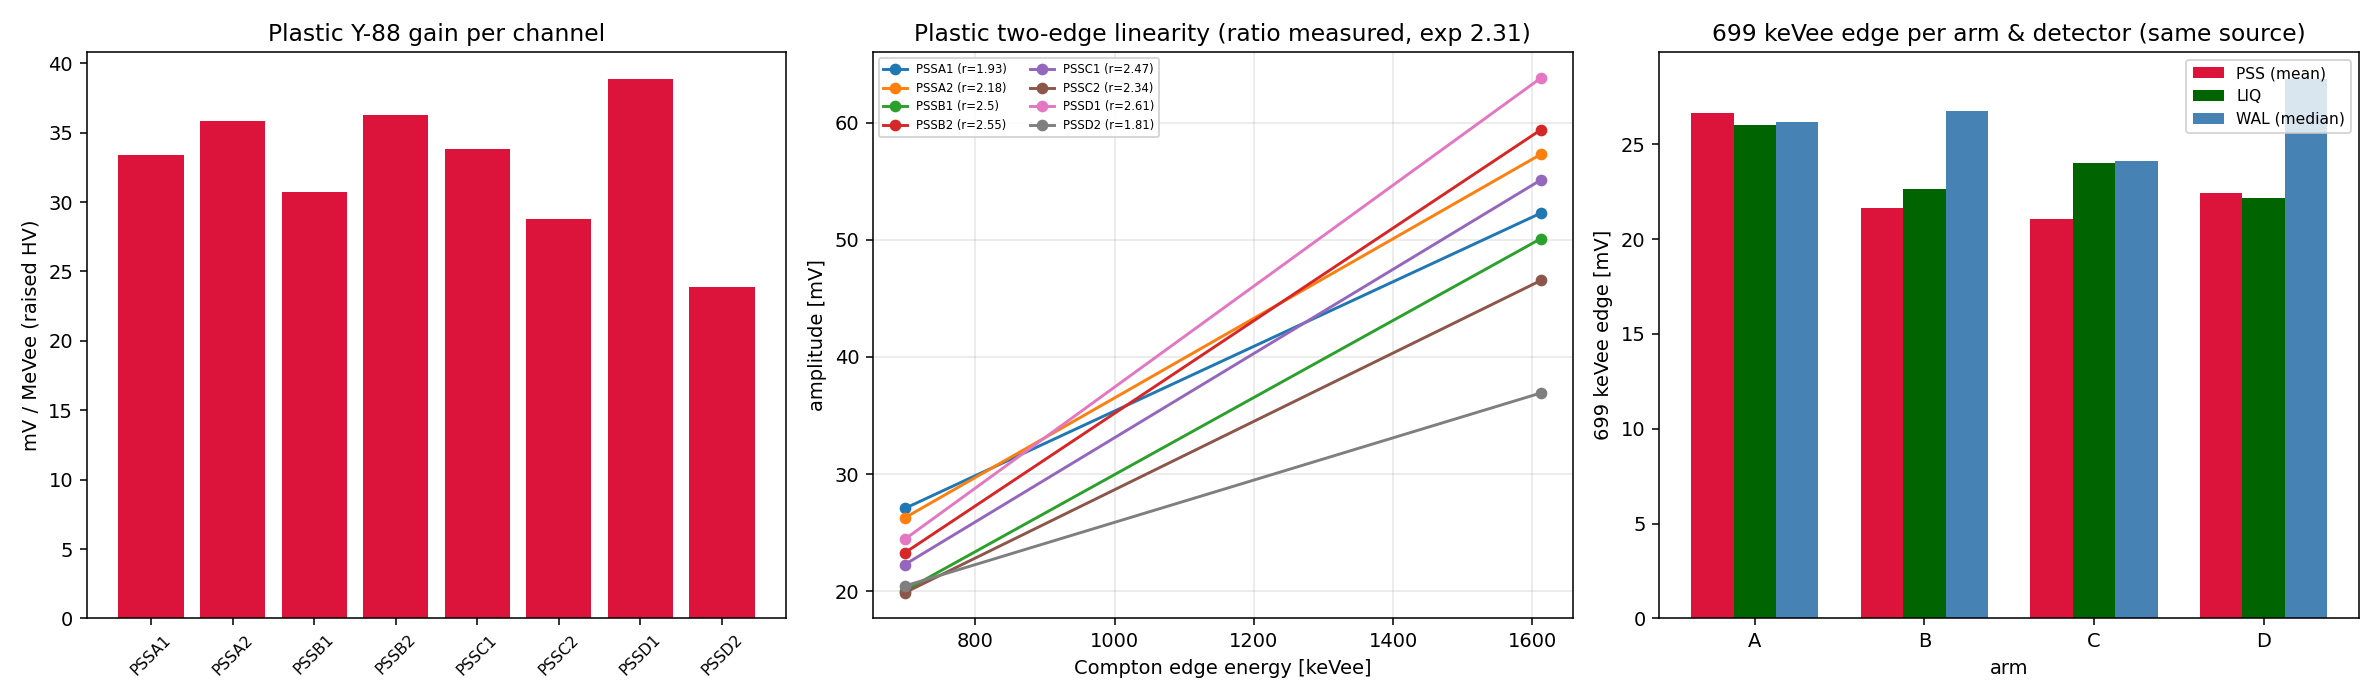
\includegraphics[width=\textwidth]{21_y88/energy_calib.png}
\column{.5\textwidth}
\begin{itemize}
\item Two edges on every plastic; measured 1612/699 ratio $\approx 2.4$
      (expect 2.31) \emph{confirms} the energy assignment.
\item Plastic gain \textbf{35--64 mV/MeVee} (HV raised for these runs).
\item \textbf{First LIQ scale}: 32--37 mV/MeVee, consistent across arms.
\item At 699 keVee all three detectors land within 21--27 mV per arm.
\end{itemize}
\end{columns}
\end{frame}

\begin{frame}{\textcolor{red}{Discrepancy \#1}: plastic MIP is mis-calibrated by $\sim$40$\times$}
\begin{columns}
\column{.55\textwidth}
\begin{itemize}
\item The Y-88 line (known 699 keVee) gives plastic gain
      \textbf{35--64 mV/MeVee}.
\item The old triples ``MIP'' (\texttt{19d}) assumed a \textbf{5.05 MeV}
      deposit and got 0.65--2.05 mV/MeV.
\item $\Rightarrow$ the triples ``MIP'' peak really sits at
      \textbf{$\sim$130 keVee}, not 5 MeV --- a \textbf{$\sim$40$\times$}
      disagreement.
\item Y-88 (BNC-T) and the 224489 MIP (FIFO) are otherwise \emph{consistent}
      once the per-PMT FIFO factor (1.13--1.65) and HV are applied.
\end{itemize}
\column{.45\textwidth}
\textbf{A real MIP in 2 cm plastic} $=$ 3.4 MeV (Landau MPV) $\to$
\textbf{120--217 mV} on the Y-88 scale.\\[1ex]
The triples never find it (next slides). \\[1ex]
\textbf{Trust Y-88}; recheck the triples MIP with a dedicated
low-rate / prompt-beam run.
\end{columns}
\end{frame}

\begin{frame}{Gain curves + Y-88 anchor $\to$ setting the HV}
\begin{columns}
\column{.6\textwidth}
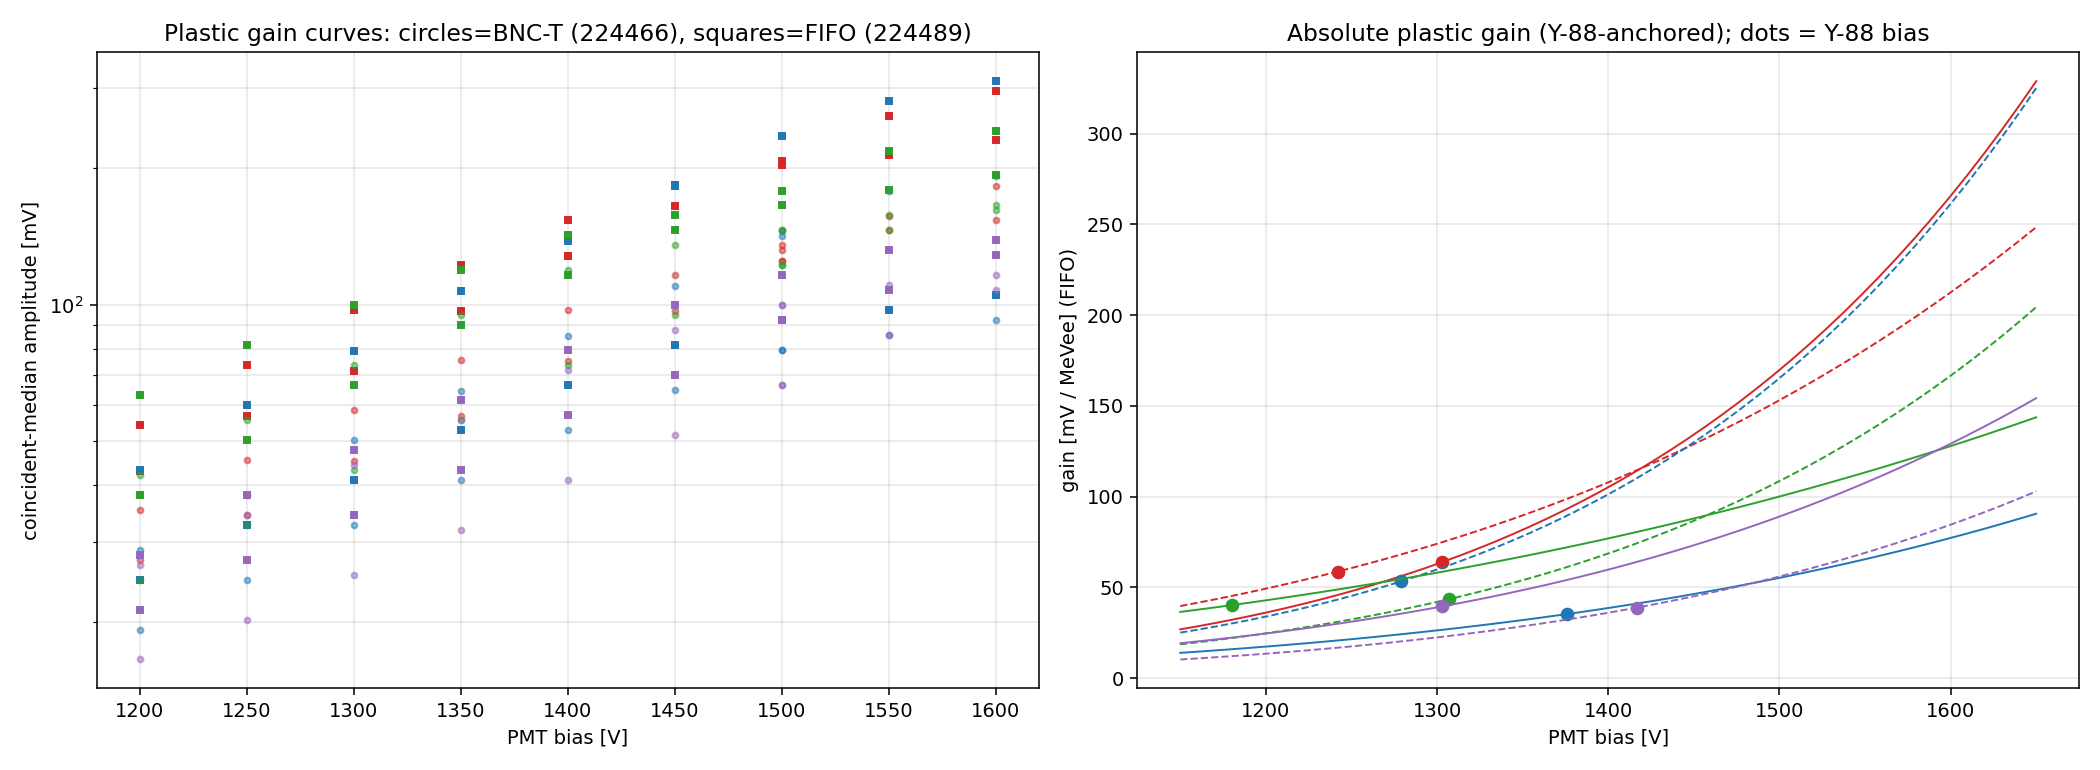
\includegraphics[width=\textwidth]{21_y88/hv_gain_curves.png}
\column{.4\textwidth}
\begin{itemize}
\item Circles = BNC-T (224466), squares = FIFO (224489); differ by the
      per-PMT FIFO factor only.
\item Y-88 pins the absolute mV/MeVee vs bias (right; dots = current bias).
\item \textbf{Equalize + scale}: per-PMT bias to put 699 keVee at a chosen mV
      (table in \texttt{HV\_GAIN\_Y88\_ANALYSIS.md}); e.g.\ 50 mV target
      $\Rightarrow$ AL 1324 \ldots\ DR 1559 V.
\end{itemize}
\end{columns}
\end{frame}

\begin{frame}{\textcolor{red}{Discrepancy \#2}: SiPM MIP differs per arm (A low)}
\begin{columns}
\column{.55\textwidth}
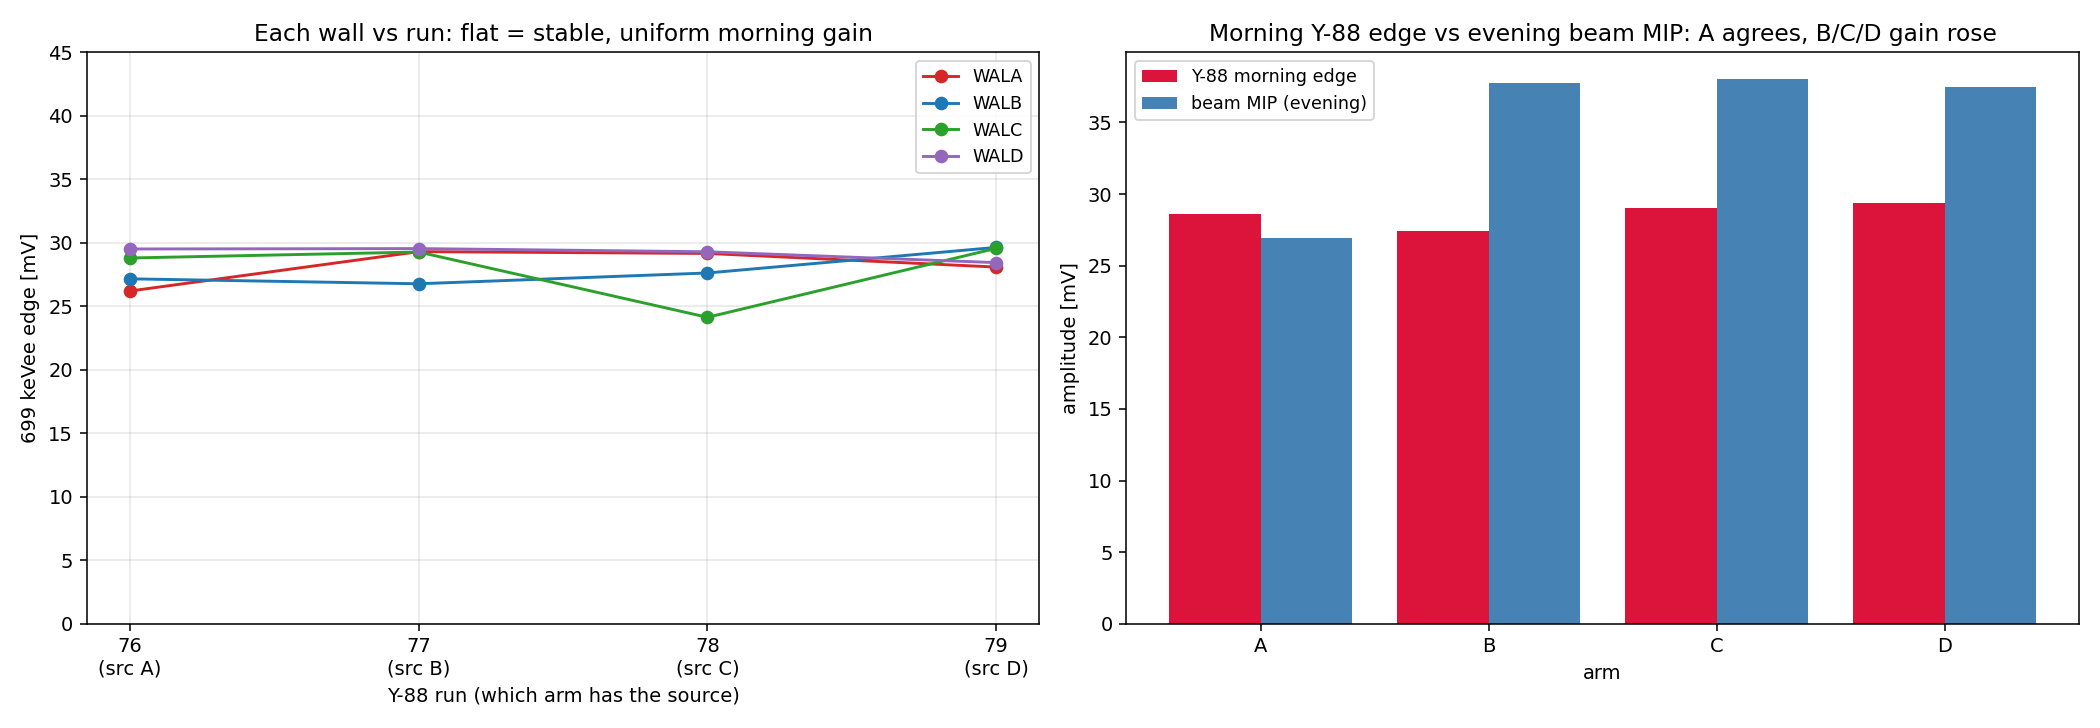
\includegraphics[width=\textwidth]{21_y88/wall_edge_stability.png}
\column{.45\textwidth}
\begin{itemize}
\item Y-88 wall edge is \textbf{uniform \& stable} across all 4 morning runs
      ($\sim$28 mV, left).
\item But the beam MIP is \textbf{arm-A-low}: A $\approx$ MIP, B/C/D
      $\sim$1.4$\times$ higher (right).
\item \textbf{Persists} in 224503 (next slide) $\Rightarrow$ not a transient.
\item Uniform Y-88 (isotropic source) $+$ non-uniform MIP (beam) $\Rightarrow$
      \textbf{geometric} (per-arm beam incidence angle $\to$ path length),
      not a gain problem. \emph{Confirm vs survey angles.}
\end{itemize}
\end{columns}
\end{frame}

\begin{frame}{Long run 224503: SiPM MIP clear, plastic MIP swamped}
\begin{columns}
\column{.55\textwidth}
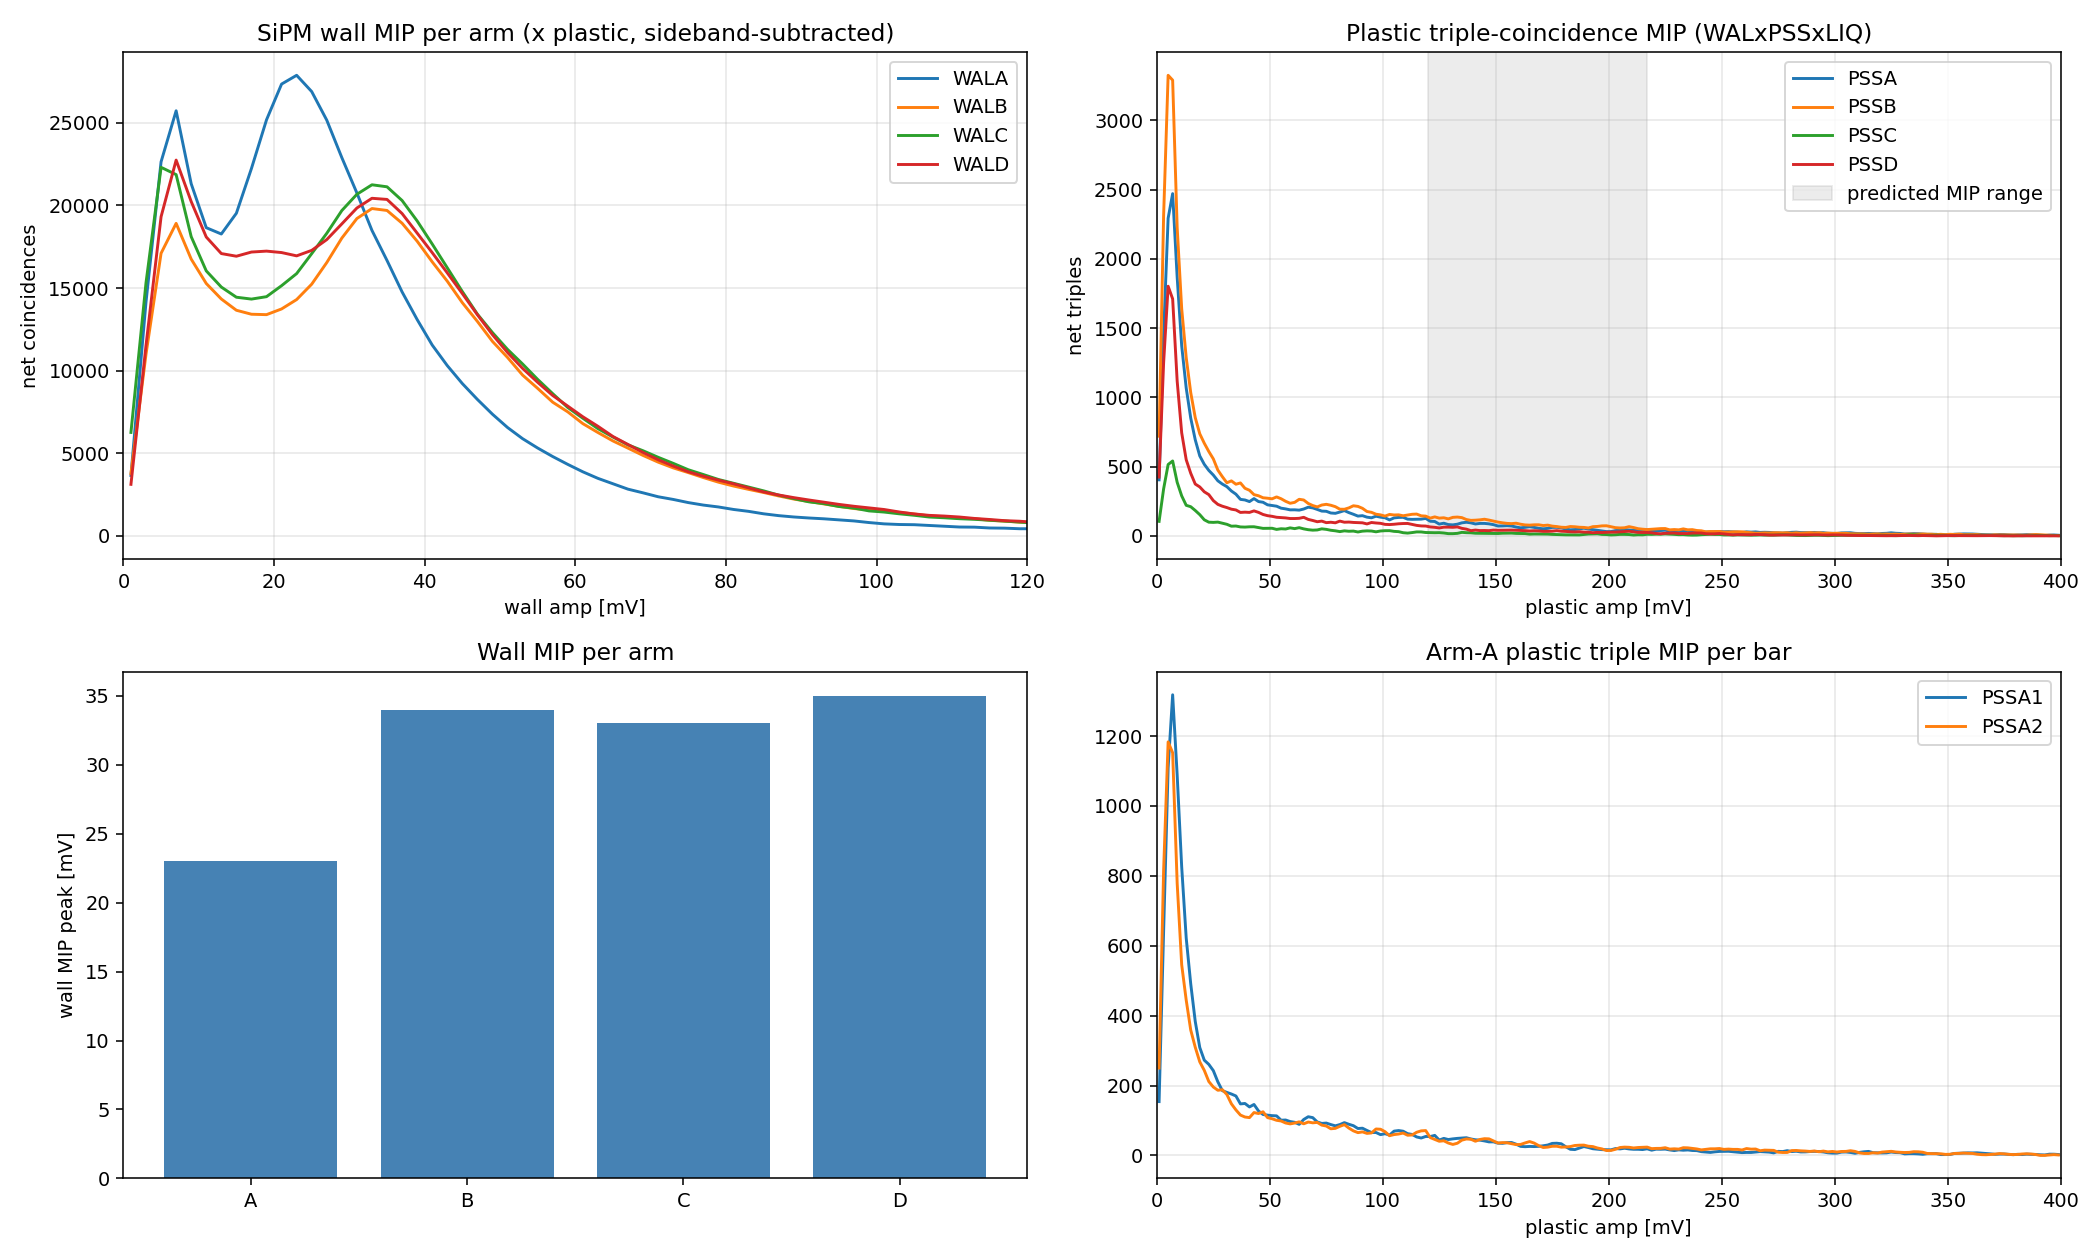
\includegraphics[width=\textwidth]{21_y88/mip_224503.png}
\column{.45\textwidth}
\begin{itemize}
\item \textbf{SiPM wall MIP} (top-left): clean bumps, WALA $\sim$23,
      B/C/D $\sim$33--35 mV --- the arm-A gap persists.
\item \textbf{Plastic triples} (top-right): net peaks at $\sim$5--7 mV, and is
      \emph{flat} across the predicted 120--217 mV MIP band.
\item Not statistics --- the plastic's huge low-energy singles rate
      ($\sim$20k hits/bunch) \textbf{swamps} the triple, and the late-tof cut
      drops prompt beam MIPs.
\item $\Rightarrow$ triples can't pull the plastic MIP from a high-rate beam run.
\end{itemize}
\end{columns}
\end{frame}

\begin{frame}{SiPM trigger thresholds (top+bottom SUM, 0.5$\times$MIP)}
\begin{columns}
\column{.56\textwidth}
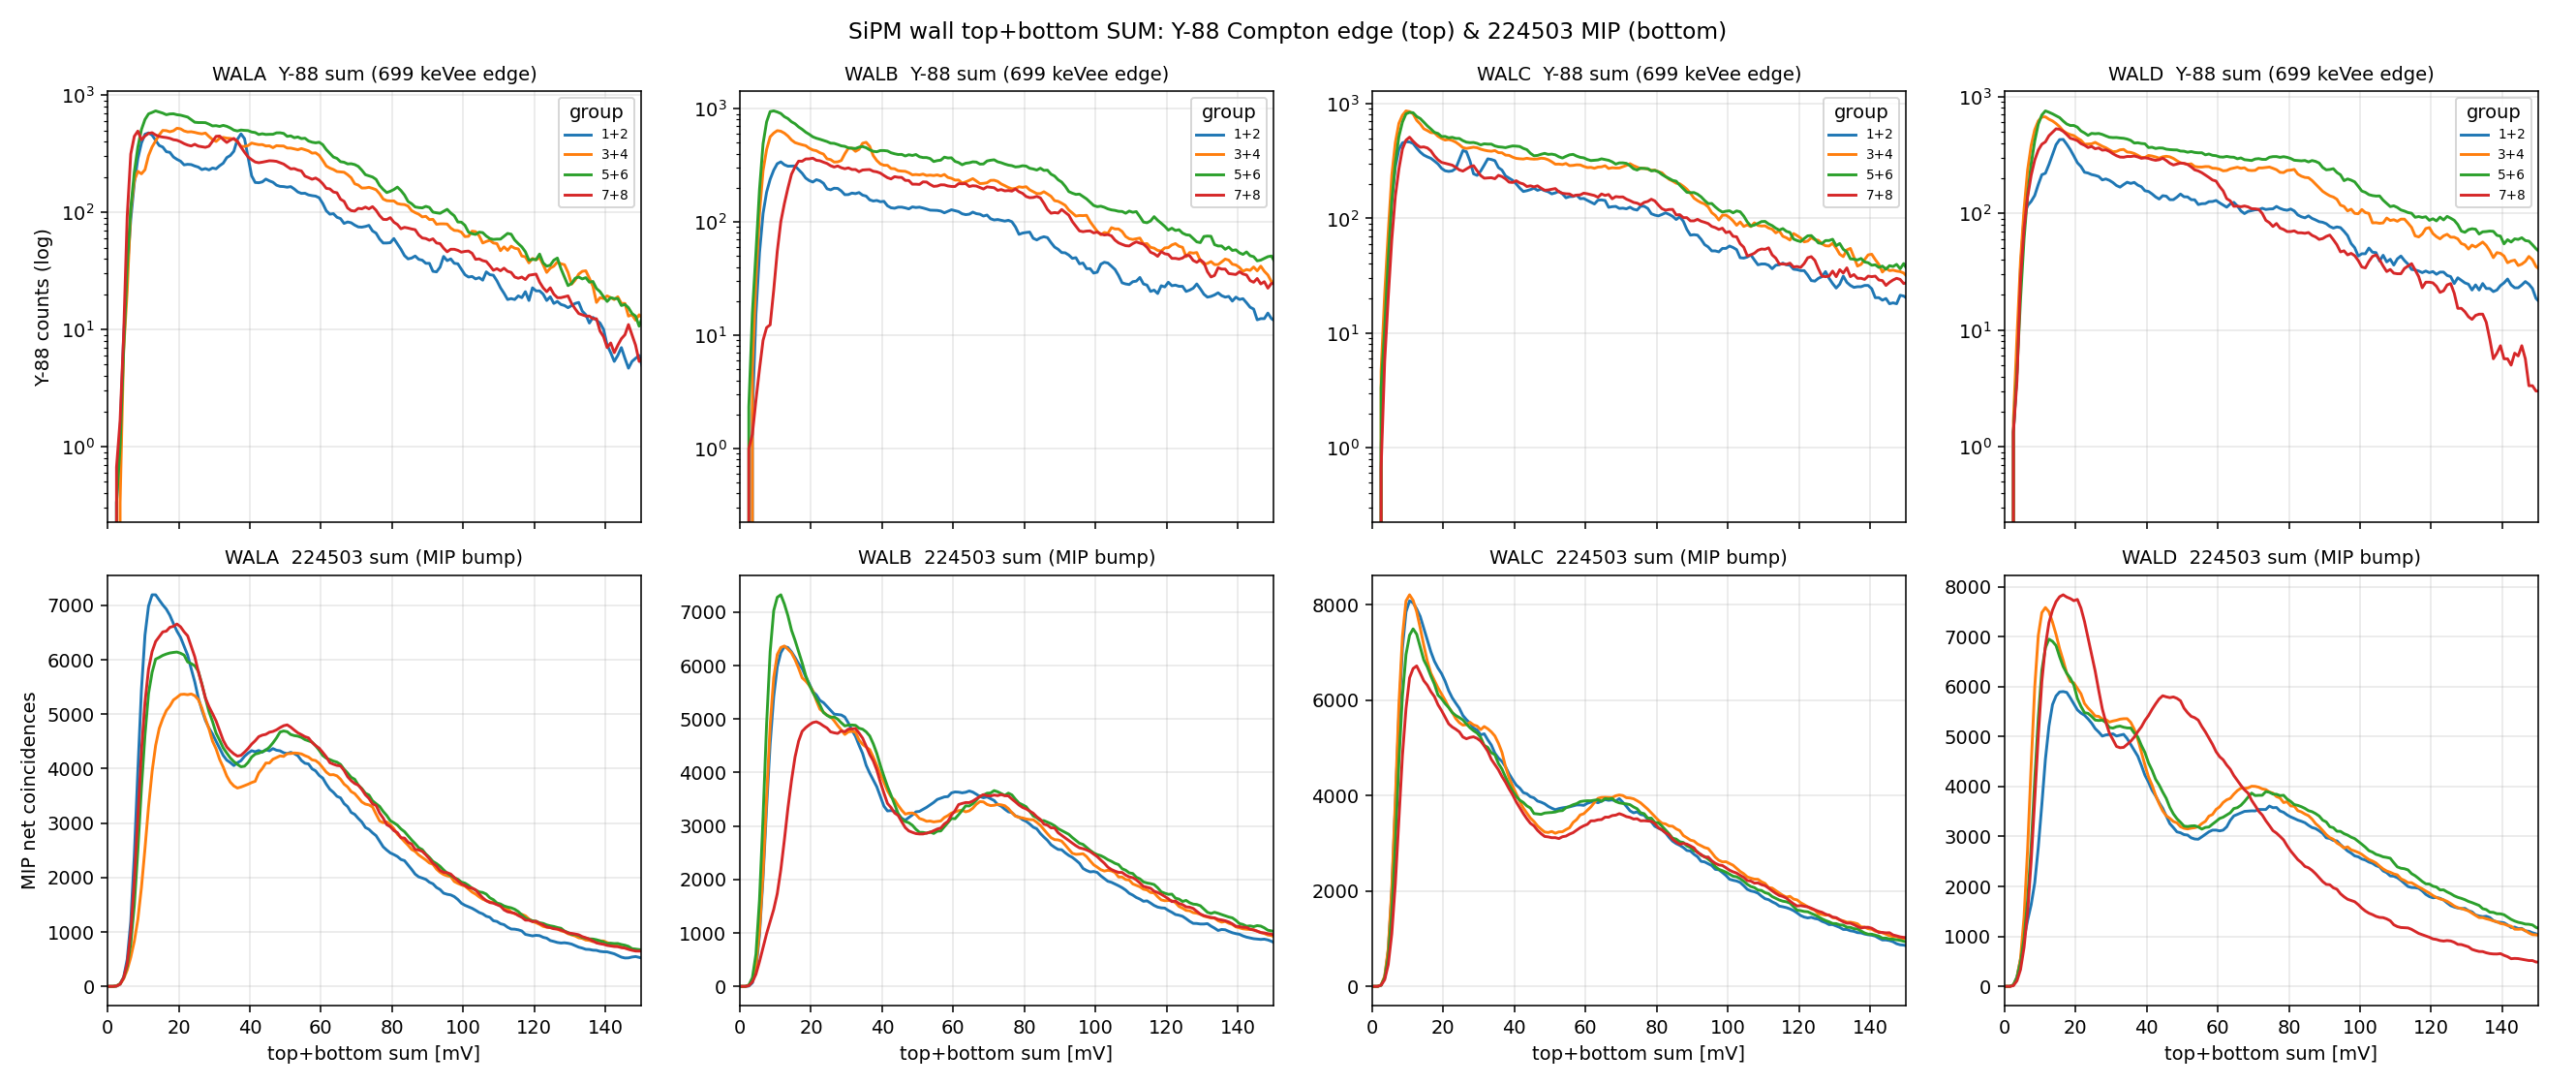
\includegraphics[width=\textwidth]{21_y88/sipm_sums.png}
\column{.44\textwidth}
Trigger fires on the top+bottom \textbf{sum} of each bar group
[(1+2)(3+4)(5+6)(7+8)]. MIP bump of the sum (bottom row), threshold $=$ half:
\vspace{1ex}
\begin{center}\small
\begin{tabular}{lcc}
\toprule
wall & MIP-sum [mV] & \textbf{thr [mV]} \\
\midrule
WALA & 50 & \textbf{25} \\
WALB & 70 & \textbf{35} \\
WALC & 67 & \textbf{34} \\
WALD & 72 & \textbf{36} \\
\bottomrule
\end{tabular}
\end{center}
\vspace{1ex}
{\small Arm A lower (Discrepancy \#2). Per-channel values in
\texttt{calib/sipm\_sum\_thresholds.json}.}
\end{columns}
\end{frame}

\begin{frame}{Plastic trigger thresholds (Y-88-anchored MIP estimate)}
No usable triple MIP $\Rightarrow$ predict the plastic MIP from the \textbf{Y-88
scale}: MIP $=$ 3.4 MeV (2 cm PVT) $\times$ gain.
\vspace{1ex}
\begin{center}\small
\begin{tabular}{lcccccccc}
\toprule
PMT & AL & AR & BL & BR & CL & CR & DL & DR \\
\midrule
predicted MIP [mV]        & 217 & 200 & 120 & 181 & 137 & 148 & 134 & 132 \\
\textbf{thr @1.7 MeV [mV]} & \textbf{109} & \textbf{100} & \textbf{60} & \textbf{91} & \textbf{68} & \textbf{74} & \textbf{67} & \textbf{66} \\
\bottomrule
\end{tabular}
\end{center}
\vspace{1ex}
\begin{itemize}
\item Threshold shown at 1.7 MeV ($\approx$ half the MIP); scales linearly ---
      pick your energy.
\item Per-channel because the current bias isn't perfectly equalized; equalize
      first (gain-curve slide) for a single common threshold ($\sim$122 mV at a
      50 mV/699-keVee target).
\item Plastic full scale $\sim$2000 mV, so huge headroom; threshold well clear
      of the $\sim$5 mV noise.
\end{itemize}
\end{frame}

\begin{frame}{Summary \& follow-ups}
\textbf{Thresholds to set now:}
\begin{itemize}
\item SiPM sums: WALA \textbf{25}, WALB \textbf{35}, WALC \textbf{34},
      WALD \textbf{36} mV (half the MIP-sum).
\item Plastics: \textbf{60--110 mV} per PMT (1.7 MeV, Y-88 scale).
\end{itemize}
\vspace{1ex}
\textbf{\textcolor{red}{Two discrepancies to follow up:}}
\begin{enumerate}
\item Plastic triples ``MIP'' is at $\sim$130 keVee, $\sim$40$\times$ below a
      real 3.4 MeV MIP --- the old \texttt{pss\_mip\_calib} energy scale is
      wrong; trust Y-88. Recheck triples with a low-rate / prompt-beam run.
\item SiPM MIP is $\sim$1.4$\times$ lower on arm A than B/C/D, persistently ---
      likely geometric (beam angle). Confirm against the survey.
\end{enumerate}
\vfill
{\small Figures \texttt{figures/21\_y88/}; calibs \texttt{calib/y88\_*.json},
\texttt{calib/sipm\_sum\_thresholds.json},
\texttt{calib/plastic\_hv\_gain\_absolute.json}.}
\end{frame}

\end{document}
